
\begin{figure}
\begin{center}
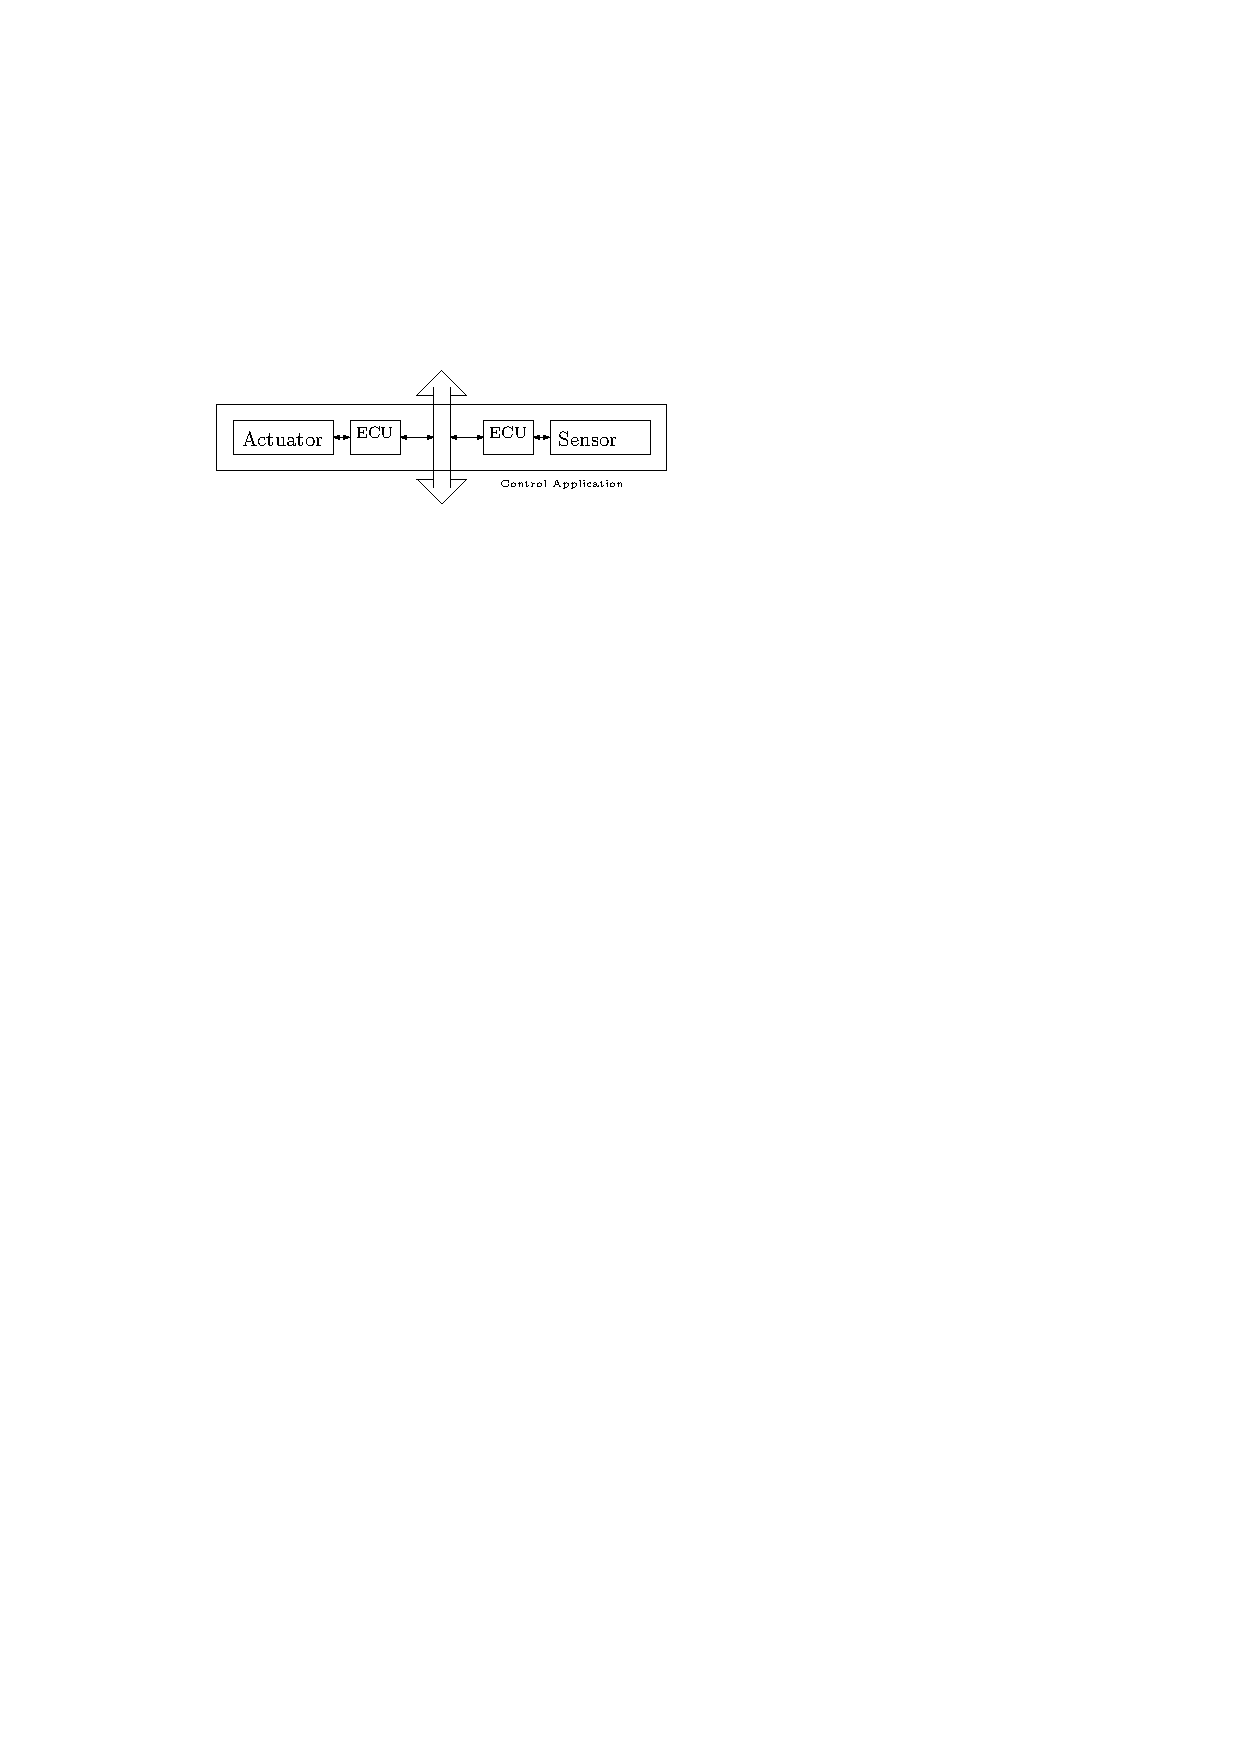
\includegraphics[width = 80mm]{system_block_diagram.pdf}
\end{center}
\caption{System Block Diagram}
\label{block_dig}
\end{figure}

The diagram of the distributed platform is given in Fig.\ref{block_dig}.
In the diagram a control application is divided into two tasks, a sensor task $T_s$ and 
an actuator task $T_a$. These tasks run on two different processors and
uses a common shared bus. A bus schedule is there to schedule messages on the bus.
When sender generates a message, it waits for the bus scheduler to get the bus
access and when bus scheduler allots bus to the message it gets transmitted to
the receiver's processor to be accessed by the receiver. Say at a particular period  
$p$, $T_a$ sends message $m_a$ to the bus and receive feedback message $m_s$ and $T_s$
accepts message $m_a$ and sends feedback message $m_s$. The timing diagram is given in Fig.\ref{tim_dig}

\begin{figure}
\begin{center}
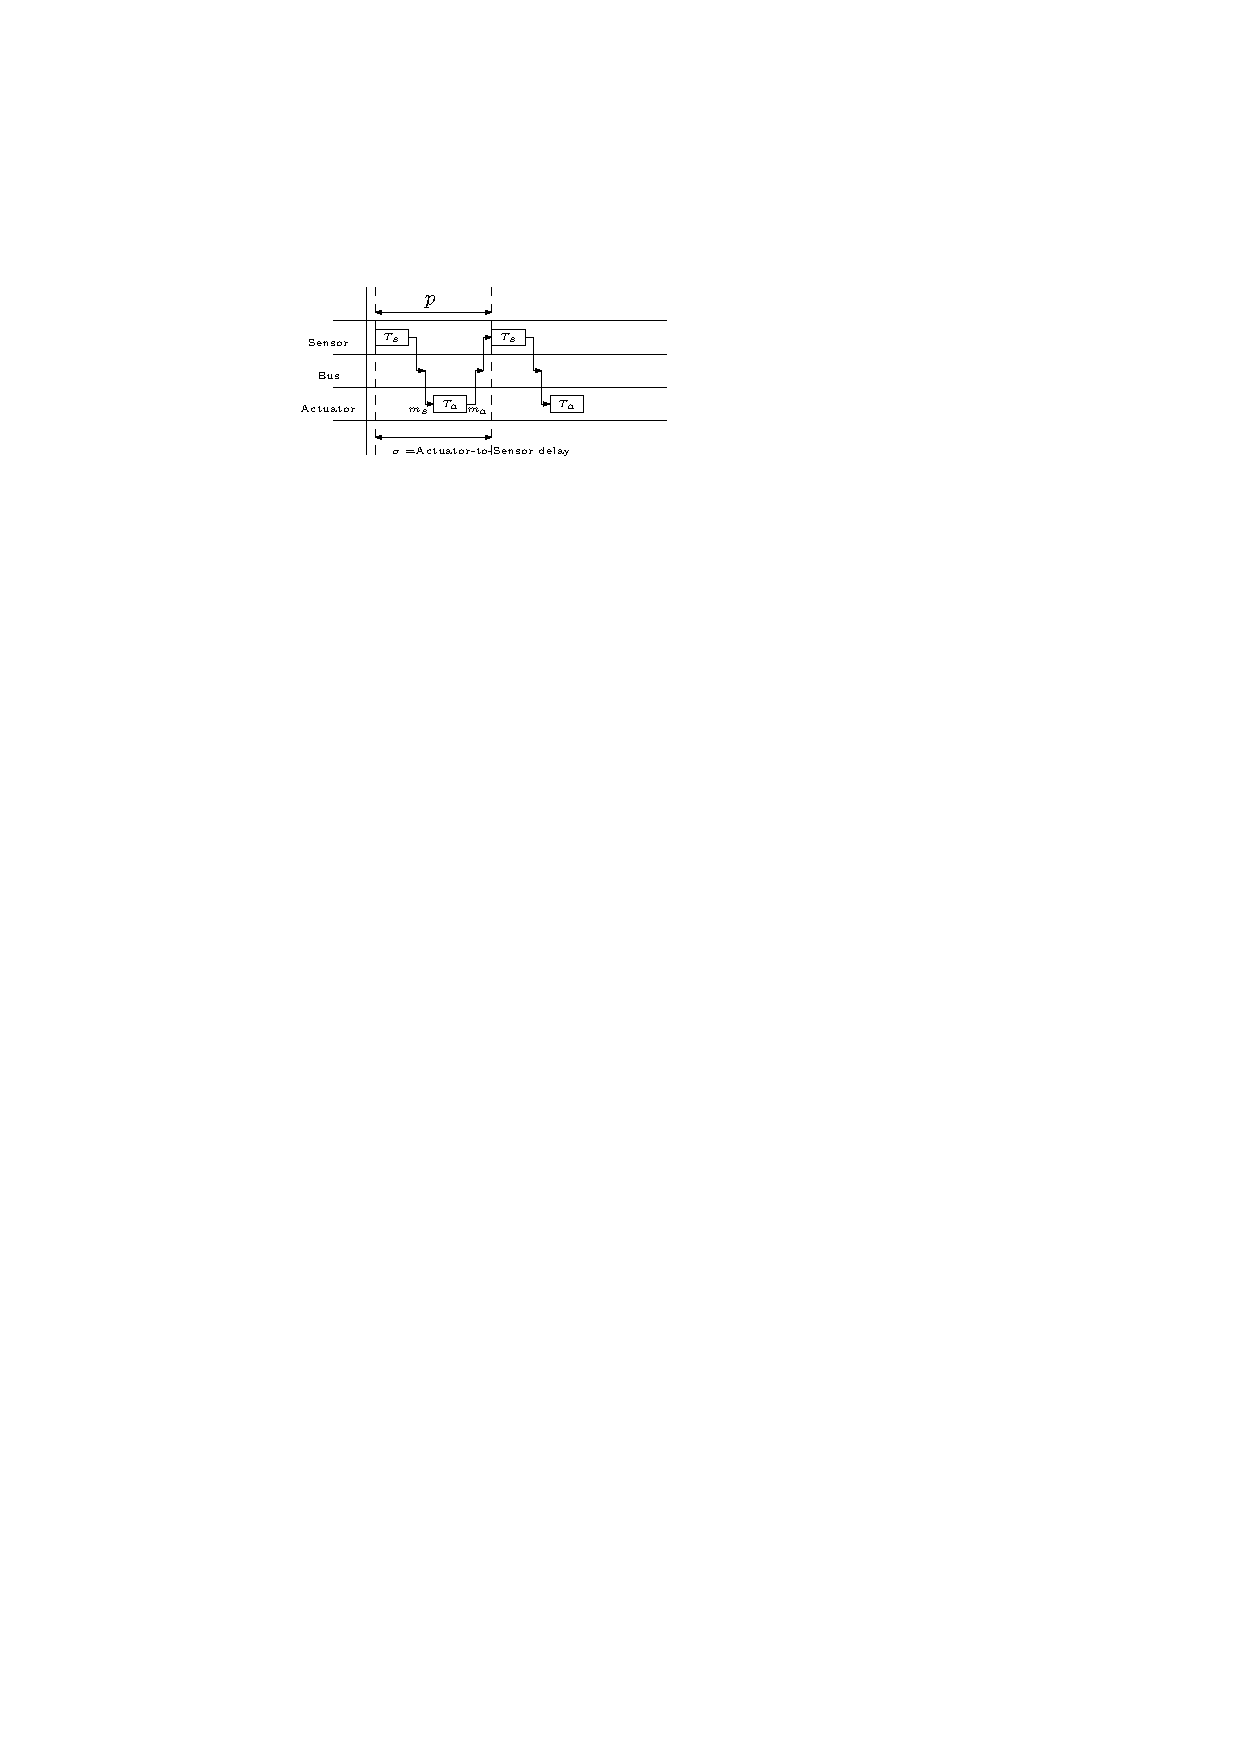
\includegraphics[width=75mm]{timing_diagram_deadline_cosntraint.pdf}
\end{center}
\caption{Timing diagram}
\label{tim_dig}
\end{figure}


The time interval between the sending message and receiving message is the
sensor-to-actuator delay denoted by $\sigma$. According to the timing diagram,
the sensor-to-actuator delay can be measured by total time needed by $T_a$
to send $m_a$ and getting feedback message $m_s$, which is some function of $m_a$,
i.e $m_a = f(m_s)$. 

From the timing diagram we can understand that $\sigma > 0$ and $\lceil{h|\sigma}\rceil >= 1$
should be true always. Such kind of constraint are common in computational process and 
control algorithms where they share a common bus in a distributed environment.


\begin{figure}
\begin{center}
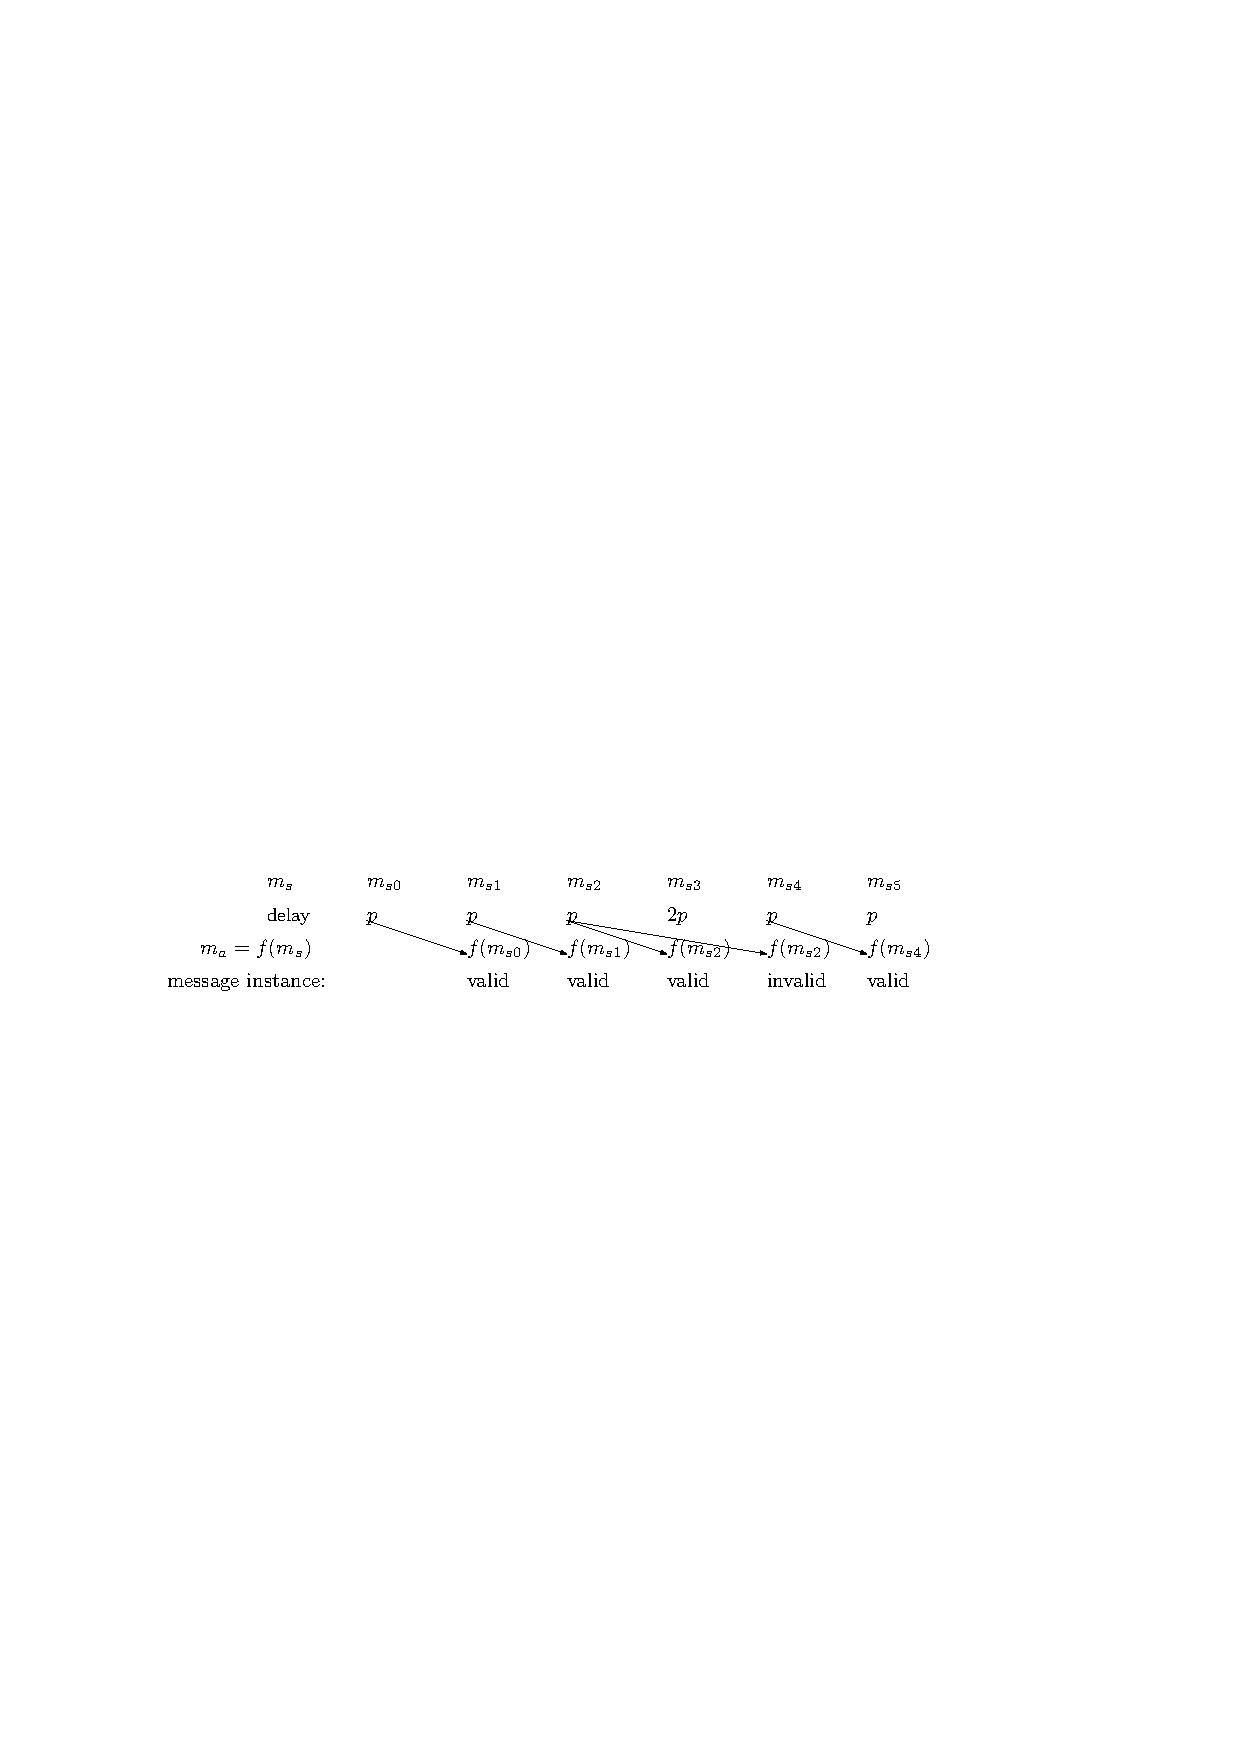
\includegraphics[width = 100mm]{timing_diagram_delay_cosntraint.pdf}
\end{center}
\caption{Timing diagram showing valid invalid sequence}
\label{tim_dig_delay}
\end{figure}

\begin{figure}
\begin{center}
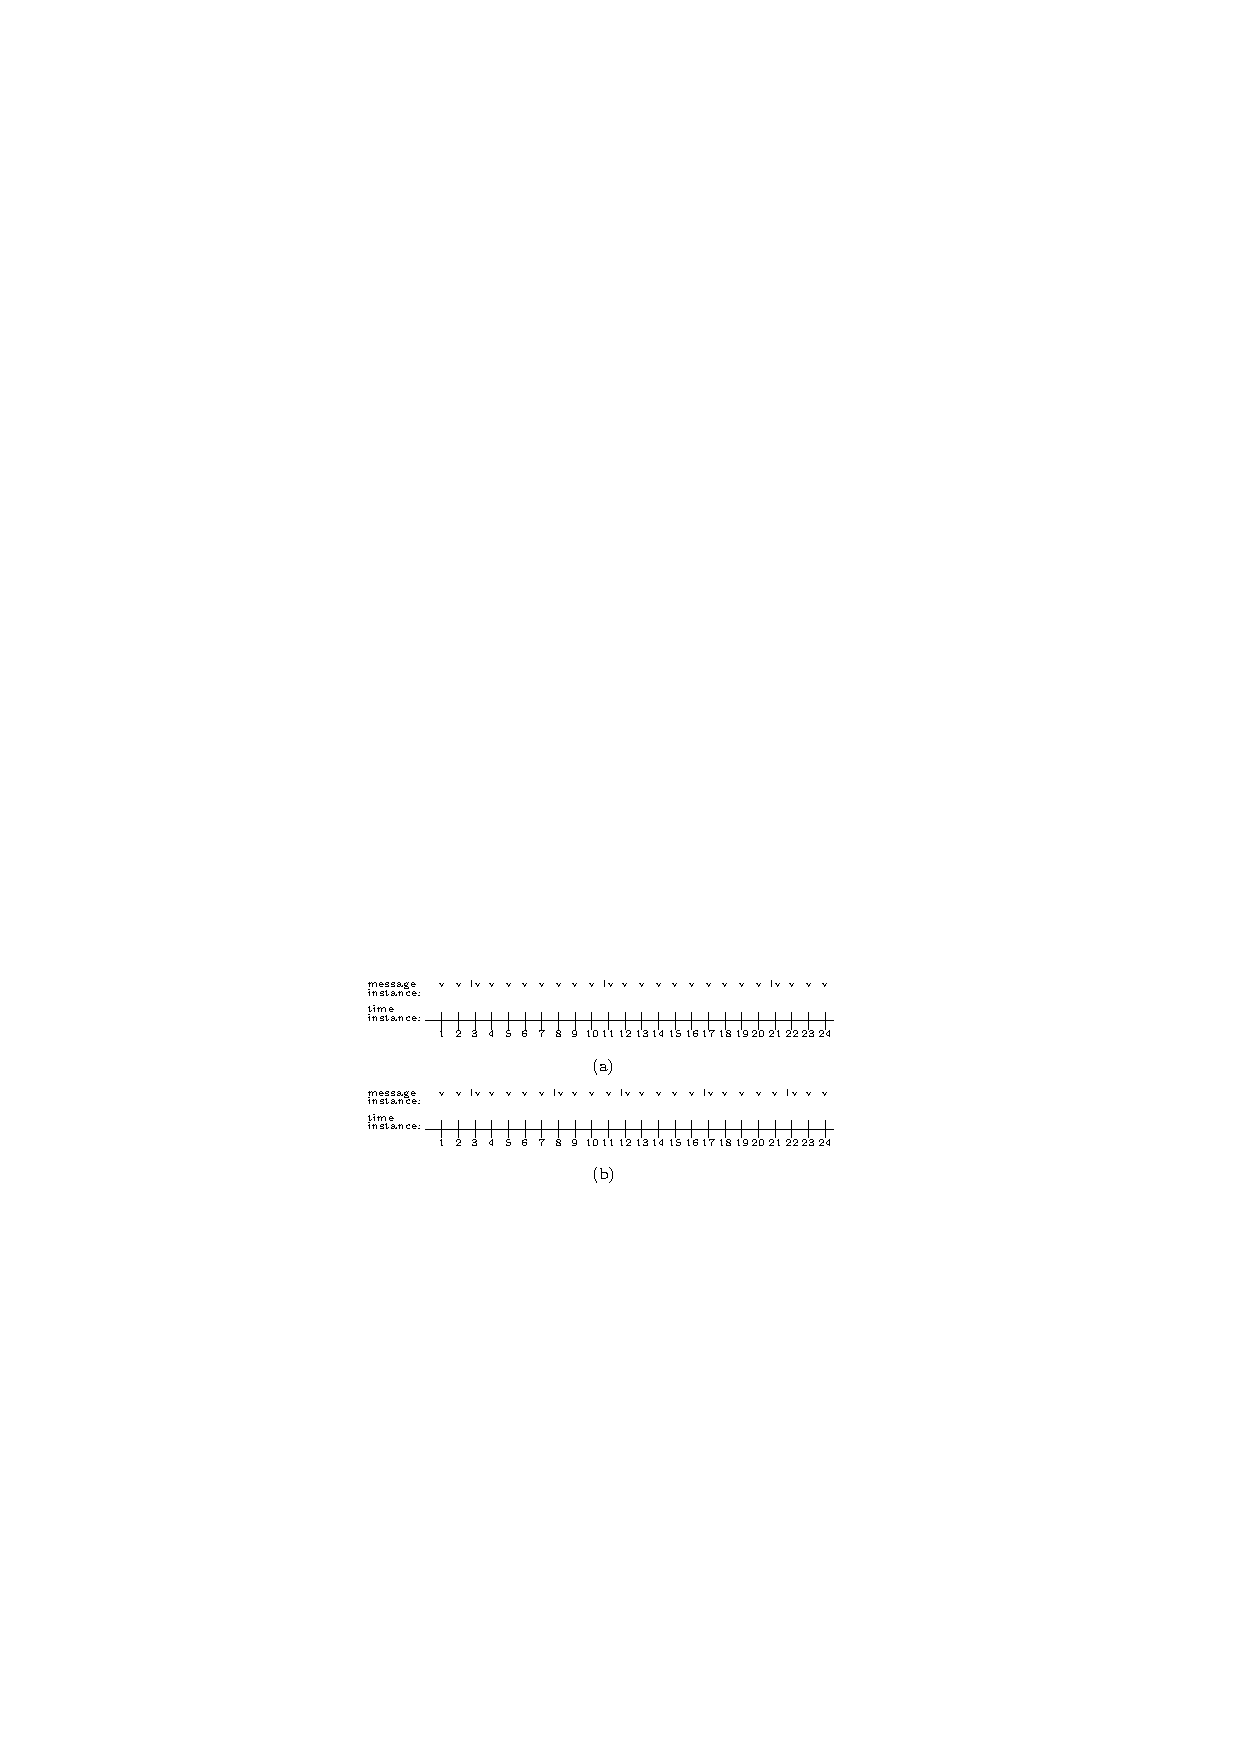
\includegraphics[width = 120mm]{valid_invalid.pdf}
\end{center}
\caption{Valid-Invalid messages from infinite sequence}
\label{tim_dig_cons}
\end{figure}


If a message is delivered within the particular period $p$ then it is called valid message but
if it is not delivered within $p$ period it becomes invalid. In the Fig.\ref{tim_dig_delay} we see that message
instance $m_{s3}$ requires $2p$ time period, so it does not get delivered within $p$ period and 
$m_{a2} = f(m_{a2})$ is delivered again which is now invalid. In Fig.\ref{tim_dig_cons}(a) we see that,
there are less number of invalid meassages but in Fig.\ref{tim_dig_cons}(b)  there are more invalid messages.
By observing the frequency of invalid messages we can say that the system got disturbance.

In such systems a sensor first sends message to a controller and the controller then sends the 
message to actuator. Each message has a deadline factor associated with depending on the computaional time(WCET).
But if for some disturbance in the system(particularly in the controller) the computaional time increases then
messages will take more time to reach the actuator. That means, they will reach after their deadline which will make them
invalid. Whether a system got disturbance can be judged by examining the number of valid-invalid message ratio.


In this problem, we are trying to capture if the invalid message counts or the valid-invalid message ratio can give any idea of 
disturbance in the system, one of the possible may be that the controller may gets replaced.








